\iftoggle{thmsty}{
\begin{definition}
\label{definition-category}
}{}
A {\it category} $\mathcal{C}$ is:
\begin{enumerate}
\item A set of objects $\Ob(\mathcal{C})$.
\item For each pair $x, y \in \Ob(\mathcal{C})$ a set of morphisms
$\Mor_\mathcal{C}(x, y)$.
\item For each triple $x, y, z\in \Ob(\mathcal{C})$ a composition
map $ \Mor_\mathcal{C}(y, z) \times \Mor_\mathcal{C}(x, y)
\to \Mor_\mathcal{C}(x, z) $, denoted $(\phi, \psi) \mapsto
\phi \circ \psi$.
\end{enumerate}
Such that these constraints are satisfied:
\begin{enumerate}
\item For every element $x\in \Ob(\mathcal{C})$ there exists a
morphism $\text{id}_x\in \Mor_\mathcal{C}(x, x)$ such that
$\text{id}_x \circ \phi = \phi$ and $\psi \circ \text{id}_x = \psi $.
\item Composition is associative, i.e., $(\phi \circ \psi) \circ \chi =
\phi \circ ( \psi \circ \chi)$.
\end{enumerate}
\iftoggle{thmsty}{
\end{definition}
}

\iftoggle{thmsty}{
\begin{definition}
\label{definition-functor}
}{}
A {\it functor} $F : \mathcal{A} \to \mathcal{B}$
between two categories $\mathcal{A}, \mathcal{B}$ is:
\begin{enumerate}
\item A map $F : \Ob(\mathcal{A}) \to \Ob(\mathcal{B})$.
\item For every $x, y \in \Ob(\mathcal{A})$ a map
$F : \Mor_\mathcal{A}(x, y) \to \Mor_\mathcal{B}(F(x), F(y))$,
denoted $\phi \mapsto F(\phi)$.
\end{enumerate}
These data should be compatible with composition and identity morphisms
in the following manner: $F(\phi \circ \psi) =
F(\phi) \circ F(\psi)$ for a composable pair $(\phi, \psi)$ of
morphisms of $\mathcal{A}$ and $F(\text{id}_x) = \text{id}_{F(x)}$.
\iftoggle{thmsty}{
\end{definition}
}

\iftoggle{thmsty}{
\begin{definition}
\label{definition-transformation-functors}
}{}
Let $F, G : \mathcal{A} \to \mathcal{B}$ be functors.
A {\it natural transformation}, or a {\it morphism of functors}
$t : F \to G$, is a collection $\{t_x\}_{x\in \Ob(\mathcal{A})}$
such that
\begin{enumerate}
\item $t_x : F(x) \to G(x)$ is a morphism in the category $\mathcal{B}$, and
\item for every morphism $\phi : x \to y$ of $\mathcal{A}$ the following
diagram is commutative
$$
\xymatrix{
F(x) \ar[r]^{t_x} \ar[d]_{F(\phi)} & G(x) \ar[d]^{G(\phi)} \\
F(y) \ar[r]^{t_y} & G(y) }
$$
\end{enumerate}
\iftoggle{thmsty}{
\end{definition}
}

\iftoggle{thmsty}{
\begin{definition}
\label{definition-products}
}{}

Let $x, y\in \Ob(\mathcal{C})$,
A {\it product} of $x$ and $y$ is
an object $x \times y \in \Ob(\mathcal{C})$
together with morphisms
$p\in \Mor_{\mathcal C}(x \times y, x)$ and
$q\in\Mor_{\mathcal C}(x \times y, y)$ such
that the following universal property holds: for
any $w\in \Ob(\mathcal{C})$ and morphisms
$\alpha \in \Mor_{\mathcal C}(w, x)$ and
$\beta \in \Mor_\mathcal{C}(w, y)$
there is a unique
$\gamma\in \Mor_{\mathcal C}(w, x \times y)$ making
the diagram
$$
\xymatrix{
w \ar[rrrd]^\beta \ar@{-->}[rrd]_\gamma \ar[rrdd]_\alpha & & \\
& & x \times y \ar[d]_p \ar[r]_q & y \\
& & x &
}
$$
commute.
\iftoggle{thmsty}{
\end{definition}
}

\iftoggle{thmsty}{
\begin{definition}
\label{definition-has-products-of-pairs}
}{}
We say the category $\mathcal{C}$ {\it has products of pairs
of objects} if a product $x \times y$
exists for any $x, y \in \Ob(\mathcal{C})$.
\iftoggle{thmsty}{
\end{definition}
}

\iftoggle{thmsty}{
\begin{definition}
\label{definition-product-category}
}{}
Let $\mathcal{A}$, $\mathcal{B}$ be categories.
The {\it product category} is the category
$\mathcal{A} \times \mathcal{B}$ with
objects
$\Ob(\mathcal{A} \times \mathcal{B}) =
\Ob(\mathcal{A}) \times \Ob(\mathcal{B})$
and
$$
\Mor_{\mathcal{A} \times \mathcal{B}}((x, y), (x', y'))
:=
\Mor_\mathcal{A}(x, x')\times
\Mor_\mathcal{B}(y, y').
$$
Composition of morphisms is defined according to components.
\iftoggle{thmsty}{
\end{definition}
}

\iftoggle{thmsty}{
\begin{definition}
\label{definition-coproducts}
}{}
Let $x, y \in \Ob(\mathcal{C})$,
A {\it coproduct}, or {\it amalgamated sum} of $x$ and $y$ is
an object $x \amalg y \in \Ob(\mathcal{C})$
together with morphisms
$i \in \Mor_{\mathcal C}(x, x \amalg y)$ and
$j \in \Mor_{\mathcal C}(y, x \amalg y)$ such
that the following universal property holds: for
any $w \in \Ob(\mathcal{C})$ and morphisms
$\alpha \in \Mor_{\mathcal C}(x, w)$ and
$\beta \in \Mor_\mathcal{C}(y, w)$
there is a unique
$\gamma \in \Mor_{\mathcal C}(x \amalg y, w)$ making
the diagram
$$
\xymatrix{
& y \ar[d]^j \ar[rrdd]^\beta \\
x \ar[r]^i \ar[rrrd]_\alpha & x \amalg y \ar@{-->}[rrd]^\gamma \\
& & & w
}
$$
commute.
\iftoggle{thmsty}{
\end{definition}
}

\iftoggle{thmsty}{
\begin{definition}
\label{definition-has-coproducts-of-pairs}
}{}
We say the category $\mathcal{C}$ {\it has coproducts of pairs
of objects} if a coproduct $x \amalg y$
exists for any $x, y \in \Ob(\mathcal{C})$.
\iftoggle{thmsty}{
\end{definition}
}

\iftoggle{thmsty}{
\begin{definition}
\label{definition-equalizers}
}{}
Suppose that $X$, $Y$ are objects of a category $\mathcal{C}$
and that $a, b : X \to Y$ are morphisms. We say a morphism
$e : Z \to X$ is an {\it equalizer} for the pair $(a, b)$ if
$a \circ e = b \circ e$ and if $(Z, e)$ satisfies the following
universal property: For every morphism $t : W \to X$
in $\mathcal{C}$ such that $a \circ t = b \circ t$ there exists
a unique morphism $s : W \to Z$ such that $t = e \circ s$.
\iftoggle{thmsty}{
\end{definition}
}

\begin{displaymath}
\xymatrix{
X
\ar@<1ex>[r]^-{a} \ar@<-1ex>[r]_-{b}
&
Y \ar[r]^-{c} \ar[dr]_-{t}
&
Z \ar@{-->}[d]^-{s}\\
& & W
}
\end{displaymath}
\iftoggle{thmsty}{
\begin{definition}
\label{definition-coequalizers}
}{}
Suppose that $X$, $Y$ are objects of a category $\mathcal{C}$
and that $a, b : X \to Y$ are morphisms. We say a morphism
$c : Y \to Z$ is a {\it coequalizer} for the pair $(a, b)$ if
$c \circ a = c \circ b$ and if $(Z, c)$ satisfies the following
universal property: For every morphism $t : Y \to W$
in $\mathcal{C}$ such that $t \circ a = t \circ b$ there exists
a unique morphism $s : Z \to W$ such that $t = s \circ c$.
\iftoggle{thmsty}{
\end{definition}
}
\begin{displaymath}
\xymatrix{
Z \ar[r]^-{c}
&
X \ar@<1ex>[r]^-{a} \ar@<-1ex>[r]_-{b}
&
Y\\
W \ar@{-->}[u]^-{s} \ar[ur]_-{t} & &
}
\end{displaymath}
\iftoggle{thmsty}{
\begin{definition}
\label{definition-initial-final}
}{}
Let $\mathcal{C}$ be a category.
\begin{enumerate}
\item An object $x$ of the category $\mathcal{C}$ is called
an {\it initial} object if for every object $y$ of $\mathcal{C}$
there is exactly one morphism $x \to y$.
\item An object $x$ of the category $\mathcal{C}$ is called
a {\it final} object if for every object $y$ of $\mathcal{C}$
there is exactly one morphism $y \to x$.
\end{enumerate}
\iftoggle{thmsty}{
\end{definition}
}

\noindent For example, in \textit{Sets} the empty set $\emptyset$ is the unique
initial object and any {\it singleton} set, a set with one element,
is a final object.

%definitions of pullbacks and pushouts
\iftoggle{thmsty}{
\begin{definition}
\label{definition-fibre-products}
}{}
Let $x, y, z\in \Ob(\mathcal{C})$,
$f\in \Mor_\mathcal{C}(x, y)$
and $g\in \Mor_{\mathcal C}(z, y)$.
A {\it fibre product} of $f$ and $g$ is
an object $x \times_y z\in \Ob(\mathcal{C})$
together with morphisms
$p\in \Mor_{\mathcal C}(x \times_y z, x)$ and
$q\in\Mor_{\mathcal C}(x \times_y z, z)$ making the diagram
$$
\xymatrix{
x \times_y z \ar[r]^{q} \ar[d]_p
&
z \ar[d]^{g}
\\
x \ar[r]^{f}
&
y
}
$$
commute, and such that the following universal property holds: for
any $w\in \Ob(\mathcal{C})$ and morphisms
$\alpha \in \Mor_{\mathcal C}(w, x)$ and
$\beta \in \Mor_\mathcal{C}(w, z)$ with
$f \circ \alpha= g\circ \beta$
there is a unique
$\gamma\in \Mor_{\mathcal C}(w, x \times_z y)$ making
the diagram
$$
\xymatrix{
w \ar[rrrd]^\beta \ar@{-->}[rrd]_\gamma \ar[rrdd]_\alpha
&
&
\\
&
&
x \times_y z \ar[d]_p \ar[r]_q
&
z \ar[d]^{g}
\\
&
&
x \ar[r]^{f}
&
z
}
$$
commute.
\iftoggle{thmsty}{
\end{definition}
}

\noindent
The dual notion to fibre products is that of push outs.

\iftoggle{thmsty}{
\begin{definition}
\label{definition-pushouts}
}{}
Let $x, y, z\in \Ob(\mathcal{C})$,
$f\in \Mor_\mathcal{C}(y, x)$
and $g\in \Mor_{\mathcal C}(y, z)$.
A {\it push out} of $f$ and $g$ is
an object $x\amalg_y z\in \Ob(\mathcal{C})$
together with morphisms
$p\in \Mor_{\mathcal C}(x, x\amalg_y z)$ and
$q\in\Mor_{\mathcal C}(z, x\amalg_y z)$ making the diagram
$$
\xymatrix{
y \ar[r]^{g} \ar[d]_f
&
z \ar[d]^{q}
\\
x \ar[r]^{p}
&
x\amalg_y z
}
$$
commute, and such that the following universal property holds:
For any $w\in \Ob(\mathcal{C})$ and morphisms
$\alpha \in \Mor_{\mathcal C}(x, w)$ and
$\beta \in \Mor_\mathcal{C}(z, w)$ with
$\alpha \circ f = \beta \circ g$ there is a unique
$\gamma\in \Mor_{\mathcal C}(x\amalg_z y, w)$ making
the diagram
$$
\xymatrix{
y \ar[r]^{g} \ar[d]_f
&
z \ar[d]^{q} \ar[rrdd]^\beta
&
&
\\
x \ar[r]^{p} \ar[rrrd]^\alpha
&
x\amalg_y z  \ar@{-->}[rrd]^\gamma
&
&
\\
&&&
w
}
$$
commute.
\iftoggle{thmsty}{
\end{definition}
}

\noindent In the category $\textit{Sets}$ a pullback is a subset of the cartesian product of two sets whereas a pushout is a quotient of the disjoint union of two sets.

%definitions of limits and colimits
Let $\mathcal{C}$ be a category. A {\it diagram} in $\mathcal{C}$ is a functor $M : \mathcal{I} \to \mathcal{C}$. $\mathcal{I}$ is the {\it index category} and $M$ is an $\mathcal{I}$-diagram. $M_i$ denotes the image of the object $i$ of $\mathcal{I}$ in $\cC$. For $\phi : i \to i' \in \Mor(I)$, $M(\phi) : M_i \to M_{i'}$.

\iftoggle{thmsty}{
\begin{definition}
\label{definition-limit}
}{}
A {\it limit} of the $\mathcal{I}$-diagram $M$ in the category
$\mathcal{C}$ is given by an object $\lim_I M$ in $\mathcal{C}$
together with morphisms $p_i : \lim_I M \to M_i$ such that
\begin{enumerate}
\item for $\phi : i \to i'$ a morphism
in $\mathcal{I}$ we have $p_{i'} =  M(\phi) \circ p_i$, and
\item for any object $W$ in $\mathcal{C}$ and any family of
morphisms $q_i : W \to M_i$ such that for all $\phi : i \to i'$
in $\mathcal{I}$ we have $q_{i'} = M(\phi) \circ q_i$ there
exists a unique morphism $q : W \to \lim_I M$ such that
$q_i = p_i \circ q$ for every object $i$ of $\mathcal{I}$.
\end{enumerate}
\iftoggle{thmsty}{
\end{definition}
}

\noindent These conditions are expressed in the commutativity of the diagram
\begin{displaymath}
\xymatrix{
&\ar[ldd]_{q_i} W \ar@{-->}[d]^{q} \ar[rdd]^{q_{i'}} & \\
& \ar[ld]^{p_i} \lim\limits_{\longleftarrow \mathcal{I}} M \ar[rd]_{p_{i'}} &\\
M_i  \ar[rr]_{M(\phi)} & & M_{i'} \\
i \ar[rr]^{\phi} & & i'
}
\end{displaymath}

\noindent
Limits $(\lim_I M, (p_i)_{i\in \Ob(\mathcal{I})})$ are unique up to unique isomorphism, if they exist at all, according to the uniqueness requirement in the definition. Products of pairs and equalizers are examples of limits. The limit over the empty diagram is a final object of $\cC$. In the category of sets all limits exist. The dual notion is that of colimits.

\iftoggle{thmsty}{
\begin{definition}
\label{definition-colimit}
}{}
A {\it colimit} of the $\mathcal{I}$-diagram $M$ in the category
$\mathcal{C}$ is given by an object $\colim_I M$ in $\mathcal{C}$
together with morphisms $s_i : M_i \to \colim_I M$ such that
\begin{enumerate}
\item for $\phi : i \to i'$ a morphism
in $\mathcal{I}$ we have $s_i = s_{i'} \circ M(\phi)$, and
\item for any object $W$ in $\mathcal{C}$ and any family of
morphisms $t_i : M_i \to W$ such that for all $\phi : i \to i'$
in $\mathcal{I}$ we have $t_i = t_{i'} \circ M(\phi)$ there
exists a unique morphism $t : \colim_I M \to W$ such that
$t_i = t \circ s_i$ for every object $i$ of $\mathcal{I}$.
\end{enumerate}
\iftoggle{thmsty}{
\end{definition}
}

\noindent These conditions are expressed in the commutativity of the diagram
\begin{displaymath}
\xymatrix{
i \ar[rr]^{\phi} & & i' \\
M_i \ar[rd]^{s_i} \ar[rdd]_{t_i} \ar[rr]^{M(\phi)} & & M_{i'} \ar[ldd]^{t_{i'}} \ar[ld]_{s_{i'}}\\
& \lim\limits_{\longrightarrow \mathcal{I}} M \ar@{-->}[d]^{t}& \\
& W &
}
\end{displaymath}
\noindent
Colimits $(\colim_I M, (s_i)_{i\in \Ob(\mathcal{I})})$ are unique up to unique isomorphism by the uniqueness requirement in the definition. Coproducts of pairs and coequalizers are examples of colimits. The colimit over an empty diagram is an initial object of $\mathcal{C}$. All colimits exist in the category of sets.

Combining the diagrams for limit and colimit (in general the objects W refer to different objects in each diagram) demonstrates the reason that limits are often referred to as {\it cones over} a diagram and colimits are referred to as {\it cocones under} a diagram
\begin{displaymath}
\xymatrix{
&\ar[ldd]_{q_i} W \ar@{-->}[d]^{q} \ar[rdd]^{q_{i'}} & \\
& \ar[ld]^{p_i} \lim\limits_{\longleftarrow \mathcal{I}} M \ar[rd]_{p_{i'}} &\\
M_i  \ar[rr]_{M(\phi)} & & M_{i'} \\
i \ar[rr]^{\phi} & & i' \\
M_i \ar[rd]^{s_i} \ar[rdd]_{t_i} \ar[rr]^{M(\phi)} & & M_{i'} \ar[ldd]^{t_{i'}} \ar[ld]_{s_{i'}}\\
& \lim\limits_{\longrightarrow \mathcal{I}} M \ar@{-->}[d]^{t}& \\
& W &
}
\end{displaymath}

We can define a category having functors as objects and natural transformations as morphisms, which is called a functor category, by recognizing that every functor $F$ comes with the {\it identity} transformation $\text{id}_F : F \to F$. In addition, given a morphism of
functors $t : F \to G$ and a morphism of functors $s : E \to F$
then the {\it composition} $t \circ s$ is defined by the rule
$$
(t \circ s)_x = t_x \circ s_x : E(x) \to G(x)
$$
for $x \in \Ob(\mathcal{A})$.
This is a morphism of functors
from $E$ to $G$.
Thus, given categories
$\mathcal{A}$ and $\mathcal{B}$ we obtain the category of functors between $\mathcal{A}$ and
$\mathcal{B}$.

\iftoggle{thmsty}{
\begin{definition}
\label{definition-equivalence-categories}
}{}
An {\it equivalence of categories}
$F : \mathcal{A} \to \mathcal{B}$ is a functor such that there
exists a functor $G : \mathcal{B} \to \mathcal{A}$ such that
the compositions $F \circ G$ and $G \circ F$ are isomorphic to the
identity functors $\text{id}_\mathcal{B}$,
respectively $\text{id}_\mathcal{A}$.
In this case we say that $G$ is a {\it quasi-inverse} to $F$.
\iftoggle{thmsty}{
\end{definition}
}

\iftoggle{thmsty}{
\begin{definition}
\label{definition-adjoint}
}{}
Let $\mathcal{C}$, $\mathcal{D}$ be categories.
Let $F : \mathcal{C} \to \mathcal{D}$ and
$G : \mathcal{D} \to \mathcal{C}$ be functors.
We say that $F$ is a {\it left adjoint} of $G$ or that
$G$ is a {\it right adjoint} to $F$, written $F \dashv G$, if there are bijections
$$
\phi_{c,d}:\Mor_\mathcal{D}(Fc, d)
\simeq
\Mor_\mathcal{C}(c, Gd)
$$
functorial in $c \in \Ob(\mathcal{C})$, and
$d \in \Ob(\mathcal{D})$.
\iftoggle{thmsty}{
\end{definition}
}

Morphisms that are associated with each other according to the bijections of an adjunction are called {\it adjoint transposes} of one another. If $g:Fc \rightarrow d$, $g \in \Mor(\cD)$ then $g^*: c \rightarrow Gd$, $g^* \in \Mor(\cC)$ is given by $\phi_{c,d}(g) = g^*$. Similarly for $f: c \rightarrow Gd$, $f \in \Mor(\cC)$ with $f^*:Fc \rightarrow d$, $f^* \in \Mor(\cD)$ is given by $\phi_{c,d}^{-1}(f) = f^*$. We see then that $g^* = f$ and $f^* = g$.

\iftoggle{thmsty}{
\begin{definition}
\label{definition-opposite}
}{}
Given a category $\mathcal{C}$ the {\it opposite category}
$\mathcal{C}^{opp}$ is the category with the same objects
as $\mathcal{C}$ but all morphisms reversed.
\iftoggle{thmsty}{
\end{definition}
}

\iftoggle{thmsty}{
\begin{definition}
\label{definition-contravariant}
}{}
Let $\mathcal{C}$, $\mathcal{S}$ be categories.
A {\it contravariant} functor $F$
from $\mathcal{C}$ to $\mathcal{S}$
is a functor $\mathcal{C}^{opp}\to \mathcal{S}$.
\iftoggle{thmsty}{
\end{definition}
}

\iftoggle{thmsty}{
\begin{definition}
\label{definition-presheaf}
}{}
Let $\mathcal{C}$ be a category.
\begin{enumerate}
\item A {\it presheaf of sets on $\mathcal{C}$}
or simply a {\it presheaf} is a contravariant functor
$F$ from $\mathcal{C}$ to $\textit{Sets}$. When $F$ is a covariant functor $F : \mathcal{C}^{opp} \rightarrow \textit{Sets}$.
\item The category of presheaves is denoted $\textit{PSh}(\mathcal{C})$.
\end{enumerate}
\iftoggle{thmsty}{
\end{definition}
}

\iftoggle{thmsty}{
\begin{definition}
\label{definition-bifunctor}
}{}
Given categories $\mathcal{C}_1$, $\mathcal{C}_2$, and $\mathcal{D}$. A {\it bifunctor} or binary functor or 2-ary functor or functor of two variables, $F$, is a functor whose domain is the product of two categories $F: \mathcal{C}_1 \times \mathcal{C}_2 \rightarrow \mathcal{D}$.
\iftoggle{thmsty}{
\end{definition}
}

\iftoggle{thmsty}{
\begin{definition}
\label{definition-hom-functor}
}{}
The {\it hom-functor} is a bifunctor defined on the product of a category $\mathcal{C}$ with its self-dual category $\mathcal{C}^{opp}$, which takes values in the category $\textit{Sets}$. Thus for a category $C$ its hom-functor is
$$
hom(-,-): \mathcal{C}^{opp} \times \mathcal{C} \rightarrow \textit{Sets},
$$
which can be curried in two ways
\begin{eqnarray*}
h^{(-)} &:& \mathcal{C}^{opp} \rightarrow \textit{Sets}^{\mathcal{C}},\\
h_{(-)} &:& \mathcal{C} \rightarrow \textit{Sets}^{\mathcal{C}^{opp}}.
\end{eqnarray*}
The hom-functor maps
\begin{enumerate}
\item objects $(c,c') \in \mathcal{C}^{opp} \times \mathcal{C}$ to the hom-set $\Mor_{\mathcal{C}} (c,c')$, which is the set of morphisms in $\mathcal{C}$ with domain $c$ and codomain $c'$.
\item morphisms
$$
(f,g):(c,c') \rightarrow (d,d') \in \Mor(\mathcal{C}^{opp} \times \mathcal{C}),
$$
where $f:d \rightarrow c \in \Mor(\mathcal{C})$ and $g:c' \rightarrow d' \in \Mor(\mathcal{C})$, to the set function
\begin{eqnarray*}
\Mor_{\mathcal{C}}(c,c') &\rightarrow& \Mor_{\mathcal{C}}(d,d')\\
(c \rightarrow c') &\mapsto& (d \rightarrow c \rightarrow c' \rightarrow d')
\end{eqnarray*}
\end{enumerate}
\iftoggle{thmsty}{
\end{definition}
}

\iftoggle{thmsty}{
\begin{definition}
\label{definition-representable-functor}
}{}
For a hom-functor $hom(-,-): \mathcal{C}^{opp} \times \mathcal{C} \rightarrow \textit{Sets}$ for $c \in \Ob(\mathcal{C})$ a covariant and contravariant functor can be derived by specializing the hom-functor to morphisms out of or into the object $c$ as
\begin{eqnarray*}
h^c \equiv hom(c,-) &:& \mathcal{C} \rightarrow \textit{Sets},\\
h_c \equiv hom(-,c) &:& \mathcal{C}^{opp} \rightarrow \textit{Sets}.
\end{eqnarray*}
Functors that are isomorphic to $h^c$ or $h_c$ are referred to as {\it corepresentable or representable functors} respectively and $c$ is their {\it representing object}. Note that $h_c \in \Ob(\textit{PSh}(\mathcal{C}))$ and the Yoneda embedding states that $h_c$ extends to a functor $PSh : \mathcal{C} \rightarrow \textit{Sets}^{\mathcal{C}^{opp}}$ that is guaranteed to be full and faithful thereby having $\mathcal{C}$ as a full subcategory of the functor category $\textit{Sets}^{\mathcal{C}^{opp}}$ by the Yoneda lemma.
\iftoggle{thmsty}{
\end{definition}
}

\begin{figure}
\noindent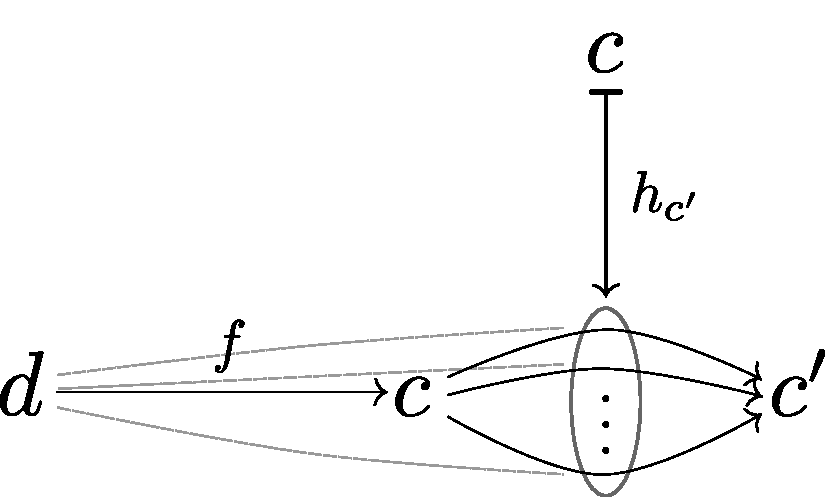
\includegraphics[width=0.7\columnwidth]{fig/hom.pdf}
\caption{The presheaf represented by $c' \in \Ob(\cC)$ is $h_{c'} : \cC^{opp} \rightarrow \textit{Sets}$. It sends objects to the set of morphisms in which they are the domain object with codomain $c'$ and morphisms $f:d \rightarrow c \in \Mor{\cC}$ to set functions $h_{c'} \circ f: \Mor_{\cC}(c,c') \rightarrow \Mor_{\cC}(d,c')$ via pre-composition.}
\label{fig:hom}
\end{figure}

The concrete action of $h_{c'}$ on objects and morphisms in $\cC$ is summarized in \ref{fig:hom}. The preceding definitions are standard category theoretic constructions. Ellerman has proposed an interpretation of adjoint functors, that demonstrates their relevance to the concept of information encoding and decoding (or sending and receiving) in the context of biological systems \cite{Ellerman2005}.

\iftoggle{thmsty}{
\begin{definition}
\label{definition-birepresentable}
}{}
A bifunctor $bif (-,-): \cC^{opp} \times \cD \rightarrow \textit{Sets}$ is said to be {\it birepresentable} if there exists a pair of functors $F:\cC^{opp} \rightleftarrows \cD:G$ where $c \in \Ob(\cC^{opp})$ and $d \in \Ob(\cD)$ gives
\begin{eqnarray*}
b^{c} \equiv bif(c,-) &:& \mathcal{D} \rightarrow \textit{Sets},\\
b_{d} \equiv bif(-,d) &:& \mathcal{C}^{opp} \rightarrow \textit{Sets}.
\end{eqnarray*}
natural in $c$ and $d$ such that $F \dashv G$. The functors $b^{c}$ and $b_{d}$ are defined on
\begin{enumerate}
\item objects for all $c_i \in \Ob(\cC^{opp})$ and for all $d_i \in \Ob(\cD)$
\begin{eqnarray*}
b^{c} (d_i) &=& \Mor_{\cD}(Fc,d_i),\\
b_{d} (c_i) &=& \Mor_{\cC^{opp}}(c_i,Gd).
\end{eqnarray*}
\item morphisms for all $f_{ij}:c_j \rightarrow c_i \in \Mor(\cC^{opp})$ and for all $g_{ij}:d_i \rightarrow d_j \in \Mor(\cD)$ as
\begin{eqnarray*}
b^{c} (g_{ij}) &:& \Mor_{\cD}(Fc,d_i) \rightarrow \Mor_{\cD}(Fc,d_j),\\
b_{d} (f_{ij}) &:& \Mor_{\cC^{opp}}(c_i,Gd) \rightarrow \Mor_{\cC^{opp}}(c_j,Gd).
\end{eqnarray*}
\end{enumerate}
\iftoggle{thmsty}{
\end{definition}
}{}




Let $\mathcal{C}$, $\mathcal{D}$ be categories.
Let $F : \mathcal{C} \to \mathcal{D}$ and
$G : \mathcal{D} \to \mathcal{C}$ be functors.
We say that $F$ is a {\it left adjoint} of $G$ or that
$G$ is a {\it right adjoint} to $F$, written $F \dashv G$, if there are bijections

$$
\phi_{c,d}:\Mor_\mathcal{D}(Fc, d)
\simeq
\Mor_\mathcal{C}(c, Gd)
$$

functorial in $c \in \Ob(\mathcal{C})$, and
$d \in \Ob(\mathcal{D})$.

Morphisms that are associated with each other according to the bijections of an adjunction are called {\it adjoint transposes} of one another.

There is a correspondence

\abovedisplayskip=0pt
\begin{align*}
g &: Fc \rightarrow d, \,\, g \in \Mor(\mathcal{D})\\
g^* &: c \rightarrow Gd, \,\, g^* \in \Mor(\mathcal{C})
\end{align*}

given by $\phi_{c,d}(g) = g^*$.
Similarly for

\begin{align*}
f &: c \rightarrow Gd, \,\, f \in \Mor(\mathcal{C})\\
f^* &: Fc \rightarrow d, \,\, f^* \in \Mor(\mathcal{D})
\end{align*}

given by $\phi_{c,d}^{-1}(f) = f^*$.
We see then that $g^* = f$ and $f^* = g$.

Consider the identity morphism $1_{Fc} \in \Mor_{\mathcal{D}}(Fc,Fc)$. The adjoint transpose of $1_{Fc}$ is the {\it unit} morphism at $c$

$$
\phi_{c,Fc}(1_{Fc})=1_{Fc}^*=\eta_c: c \rightarrow GFc
$$

where $\eta_c \in \Mor_{\mathcal{C}}(c,GFc)$, which, when taken to be natural in $c \in \Ob(\mathcal{C})$, gives the natural transformation

$$
\eta : 1_{\mathcal{C}} \Rightarrow GF
$$

Consider the identity morphism $1_{Gd} \in \Mor_{\mathcal{C}}(Gd,Gd)$. The adjoint transpose of $1_{Gd}$ is the {\it counit} morphism at $d$

$$
\phi_{Gd,d}^{-1}(1_{Gd})=1_{Gd}^*=\epsilon_d: FGd \rightarrow d
$$

where $\epsilon_d \in \Mor_{\mathcal{D}}(d,FGd)$, which, when natural in $d$, gives the natural transformation

$$
\epsilon: FG \Rightarrow 1_{\mathcal{D}}
$$

We can then give an alternative definition of adjoint functors in terms of the unit natural transformation (dually the counit natural transformation) as
\begin{align*}
F & \colon \mathcal{C} \rightleftarrows \mathcal{D} \colon G\\
\eta & \colon 1_{\mathcal{C}} \rightarrow GF
\end{align*}
where for any $c \in \Ob (\mathcal{C})$, $d \in \Ob (\mathcal{D})$, and $f \colon c \rightarrow Gd \in \Mor(\mathcal{C})$ there exists a unique $g \colon Fc \rightarrow d \in \Mor(\mathcal{D})$ such that $f = Gg \circ \eta_c$

		$$
					\xymatrix{
					c \ar[r]^{\eta_c} \ar[dr]_{f} & G F c \ar[d]^{G g} & F c \ar@{.>}[d]^{g}\\
					& G d & d}
		$$

		$$
			\frac{c \longrightarrow Gd}{Fc \longrightarrow d}
		$$

We can then give an alternative definition of adjoint functors in terms of the counit natural transformation (dually the unit natural transformation) as
$$
F \colon \mathcal{C} \rightleftarrows \mathcal{D} \colon G
$$
$$
\epsilon \colon FG \rightarrow 1_{\mathcal{C}}
$$
where for any $c \in \Ob (\mathcal{C})$, $d \in \Ob (\mathcal{D})$, and $g \colon Fc \rightarrow d \in \Mor(\mathcal{D})$ there exists a unique $f \colon c \rightarrow Gd \in \Mor(\mathcal{C})$ such that $g = \epsilon_D \circ Ff$

$$
			\xymatrix{
			& F c \ar[d]^{F f} \ar[dl]_{g} & c \ar@{.>}[d]^{f}\\
			d & F G d \ar[l]^{\epsilon_d} & G d}
$$

		$$
			\frac{Fc \longrightarrow d}{c \longrightarrow Gd}
		$$


\begin{align*}
- \times Z: \mathcal{C} & \rightleftarrows \mathcal{C}: (-)^Z\\
\Mor_{\mathcal{C}}(X \times Z, Y) & \cong  \Mor_{\mathcal{C}}(X, Y^Z)
\end{align*}

	\begin{center}
	Let $\Pi_Z = - \times Z$ and $E^Z = (-)^Z$
	\end{center}

			$$
			\xymatrix{
			& \Pi_Z X \ar[d]^{\Pi_Z \bar{f}} \ar[dl]_{f} & X \ar@{.>}[d]^{\bar{f}}\\
			Y & \Pi_Z E_Z Y \ar[l]^{\epsilon_Y} & E_Z Y}
			$$

			$$
			\xymatrix{
			& X \times Z \ar[d]^{\bar{f} \times 1_Z} \ar[dl]_{f} & X \ar@{.>}[d]^{\bar{f}}\\
			Y & Y^Z \times Z \ar[l]^{\epsilon_Y} & Y^Z}
			$$

\begin{align*}
- \times Z: \mathcal{C} & \rightleftarrows \mathcal{C}: (-)^Z\\
\Mor_{\mathcal{C}}(X \times Z, Y) & \cong  \Mor_{\mathcal{C}}(X, Y^Z)
\end{align*}

	\begin{center}
	Let $\Pi_Z = - \times Z$ and $E^Z = (-)^Z$
	\end{center}
\
			$$
			\xymatrix{
			& X \times Z \ar[d]^{\bar{f} \times 1_Z} \ar[dl]_{f} & X \ar@{.>}[d]^{\bar{f}}\\
			Y & Y^Z \times Z \ar[l]^{\epsilon_Y} & Y^Z}
			$$

		$$
			\frac{X \times Z \longrightarrow Y}{X \longrightarrow Y^Z}
		$$
		the counit is the evaluation map
		$$
			\epsilon_Y = ev_Y \colon Y^Z \times Z \longrightarrow Y
		$$



\begin{align*}
- \times Z: \mathcal{C} & \rightleftarrows \mathcal{C}: (-)^Z\\
\Mor_{\mathcal{C}}(X \times Z, Y) & \cong  \Mor_{\mathcal{C}}(X, Y^Z)
\end{align*}

	\begin{center}
	Let $\Pi_Z = - \times Z$ and $E^Z = (-)^Z$
	\end{center}

			$$
			\xymatrix{
			& \Pi_Z X \ar[d]^{\Pi_Z \bar{f}} \ar[dl]_{f} & X \ar@{.>}[d]^{\bar{f}}\\
			Y & \Pi_Z E_Z Y \ar[l]^{\epsilon_Y} & E_Z Y}
			$$

			$$
			\xymatrix{
			& X \times Z \ar[d]^{\bar{f} \times 1_Z} \ar[dl]_{f} & X \ar@{.>}[d]^{\bar{f}}\\
			Y & Y^Z \times Z \ar[l]^{\epsilon_Y} & Y^Z}
			$$

